\subsection{Modal analysis}
\label{sub:modal_analysis}

To understand how the structure behaves when excited by a force, it is necessary to calculate the natural frequencies and the mode shapes of the system.

As usual, the natural frequencies are the eigenvalues of the system, while the mode shapes are the eigenvectors.
Since we are dealing with a discretized system, we can expect as many natural frequencies as the number of degrees of freedom of the system.

In this phase, we can ignore the damping matrix, since its contribution is negligible in the calculation of the natural frequencies and mode shapes, so that the eigenvalues problem to be solved became:

\begin{equation}
    [M] \ddot{X} + [0] \dot{X} + [K] X = 0
\end{equation}

Which indeed brings to the standard eigenvalues problem:

\begin{equation}
    (\omega^2 [I] - [M_{FF}]^{-1} [K_{FF}]) X = 0
\end{equation}

Solvable in \texttt{MATLAB} with the following code:

\begin{lstlisting}[language=Matlab]

    [M, K] = assembly(incid, l, m, EA, EJ, gamma, idb);
    C = 1e-1 * M + 2.0e-4 * K;

    M_FF = M(1:ndof, 1:ndof);
    C_FF = C(1:ndof, 1:ndof);
    K_FF = K(1:ndof, 1:ndof);

    [mode_shapes, omega_square] = eig(M_FF\K_FF);
    omega_nat = sqrt(diag(omega_square));

\end{lstlisting}

As we have said before, from the code above we expect to have as many natural frequencies as the number of degrees of freedom of the system.
However, we always have to keep in mind the real physical representation of the problem.
In this case, the model represents a crane, which is a machine that typically works or is subjected to forces having a low frequency range.
As suggested by the assignment, our interest is in the $0-8 [Hz]$ frequency range.

Therefore, it's reasonable to expect that just the firsts few natural frequencies are significant, while for the others (even if present also in the real structure) is difficult that they will be excited by the forces acting on the crane and so we can consider them as negligible.

In the following, we will show the first four mode shapes of the system and the corresponding natural frequencies.

\begin{figure}[H]
    \begin{minipage}[b]{0.45\textwidth}
        \centering
        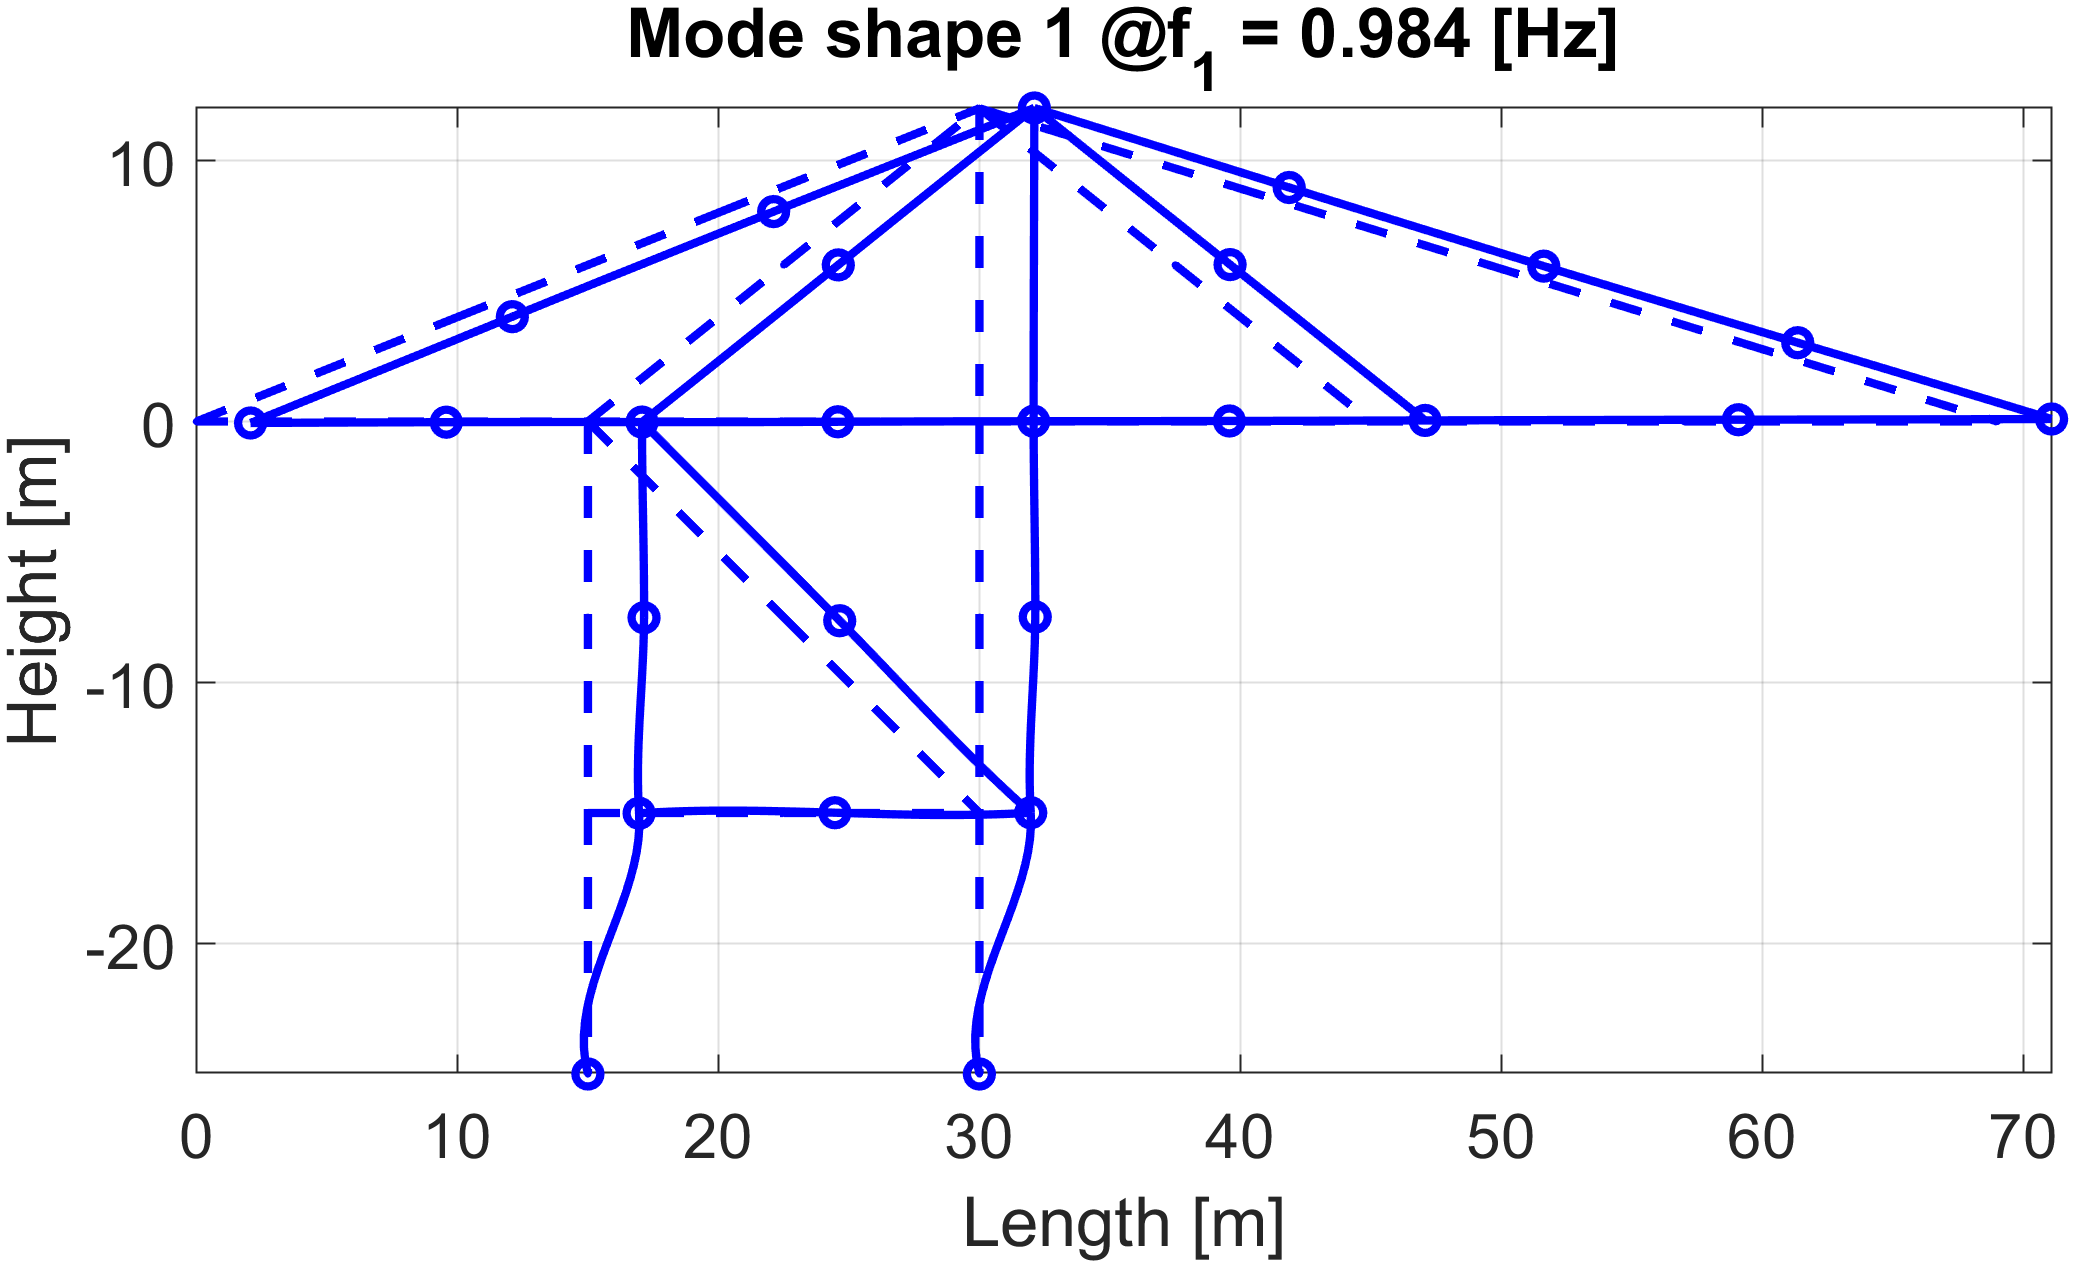
\includegraphics[width=\textwidth]{img/MATLAB/ModeShapes/Mode_01.png}
    \end{minipage}
    \hfill
    \begin{minipage}[b]{0.45\textwidth}
        \centering
        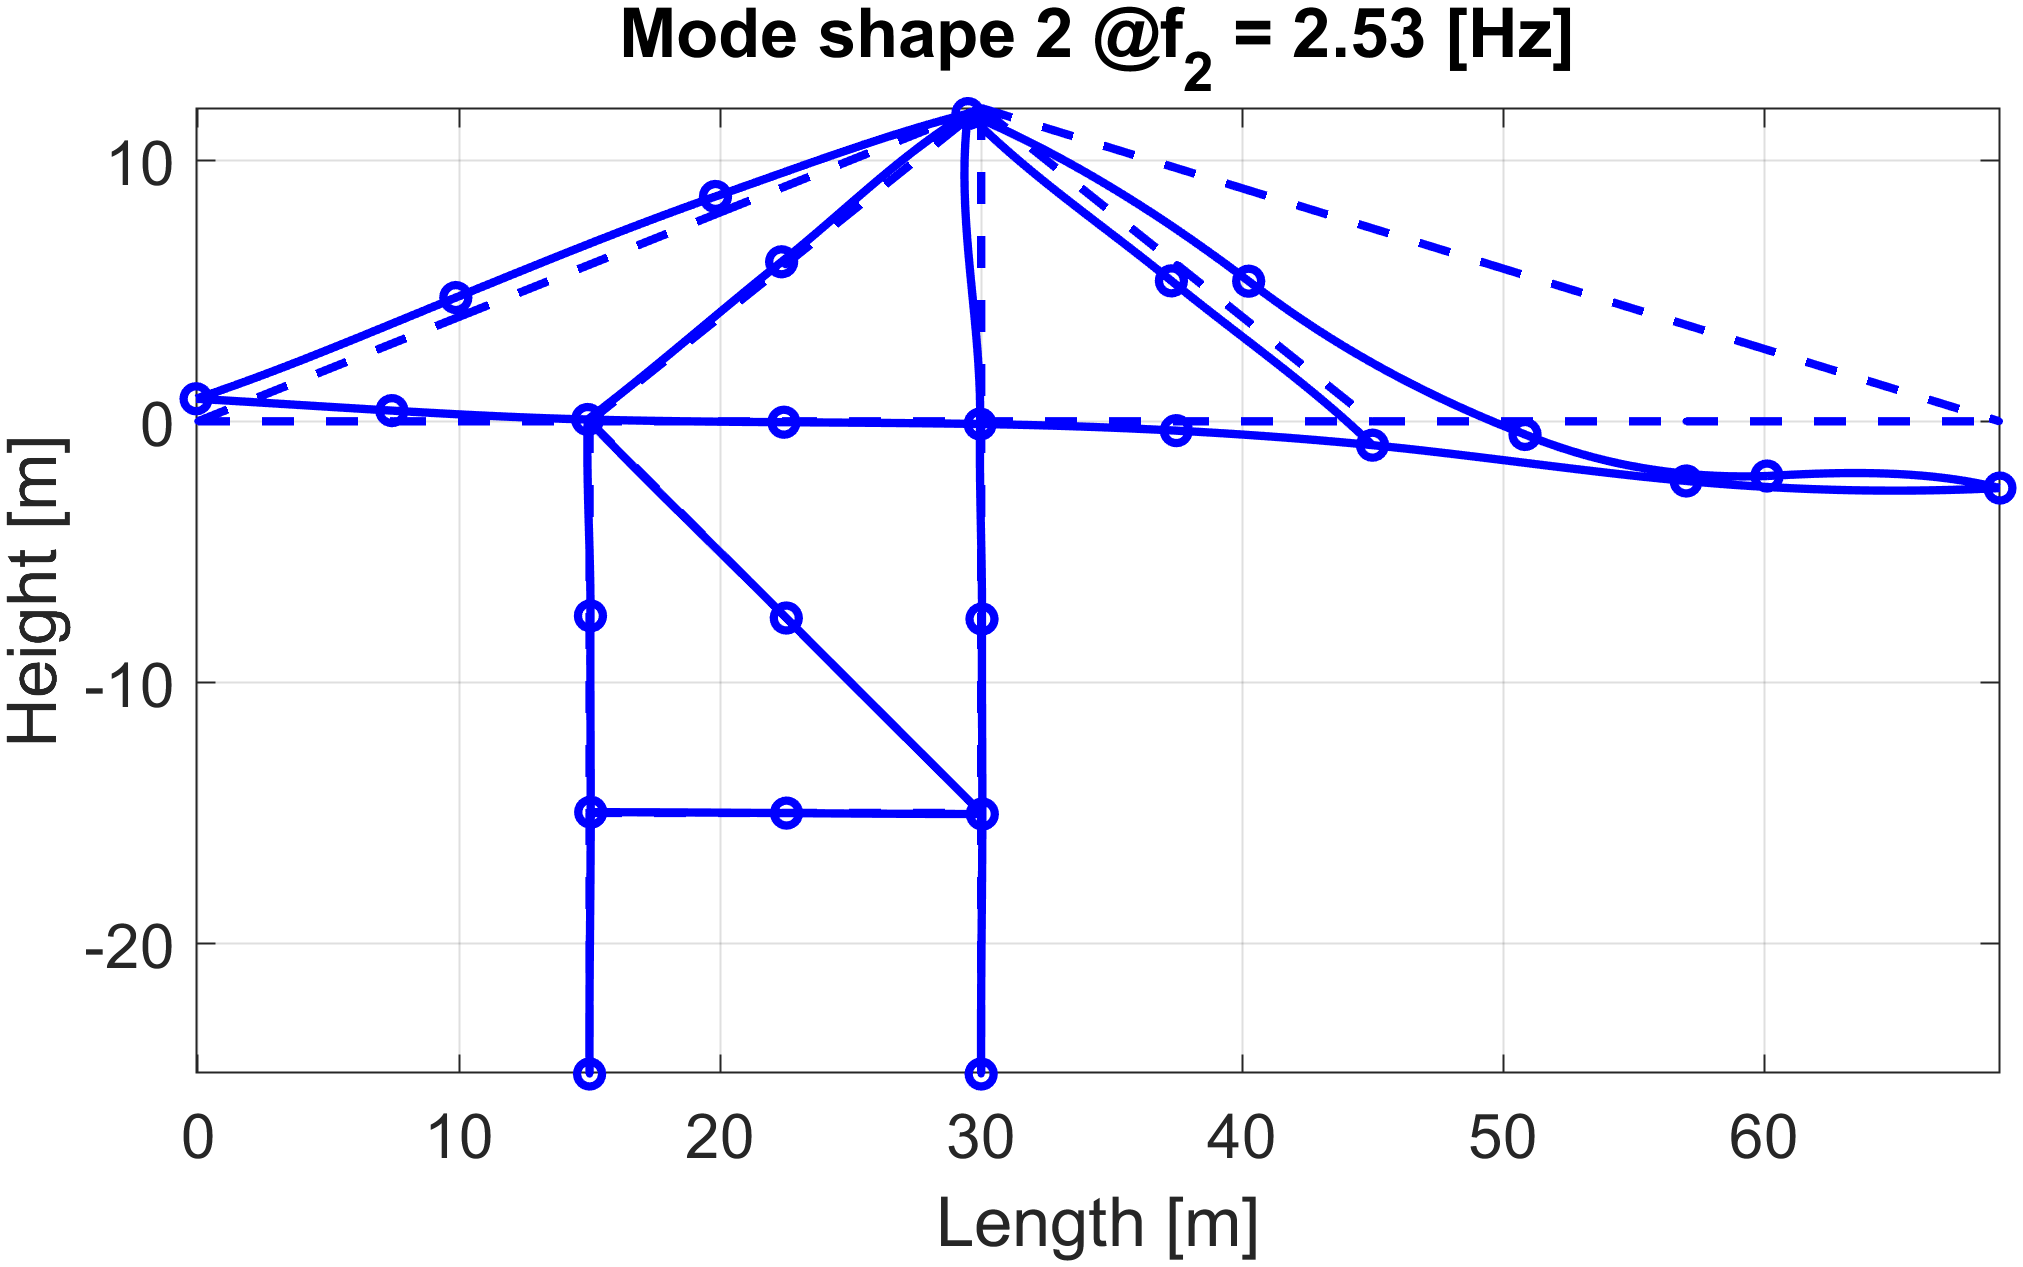
\includegraphics[width=\textwidth]{img/MATLAB/ModeShapes/Mode_02.png}
    \end{minipage}
    \begin{minipage}[b]{0.45\textwidth}
        \centering
        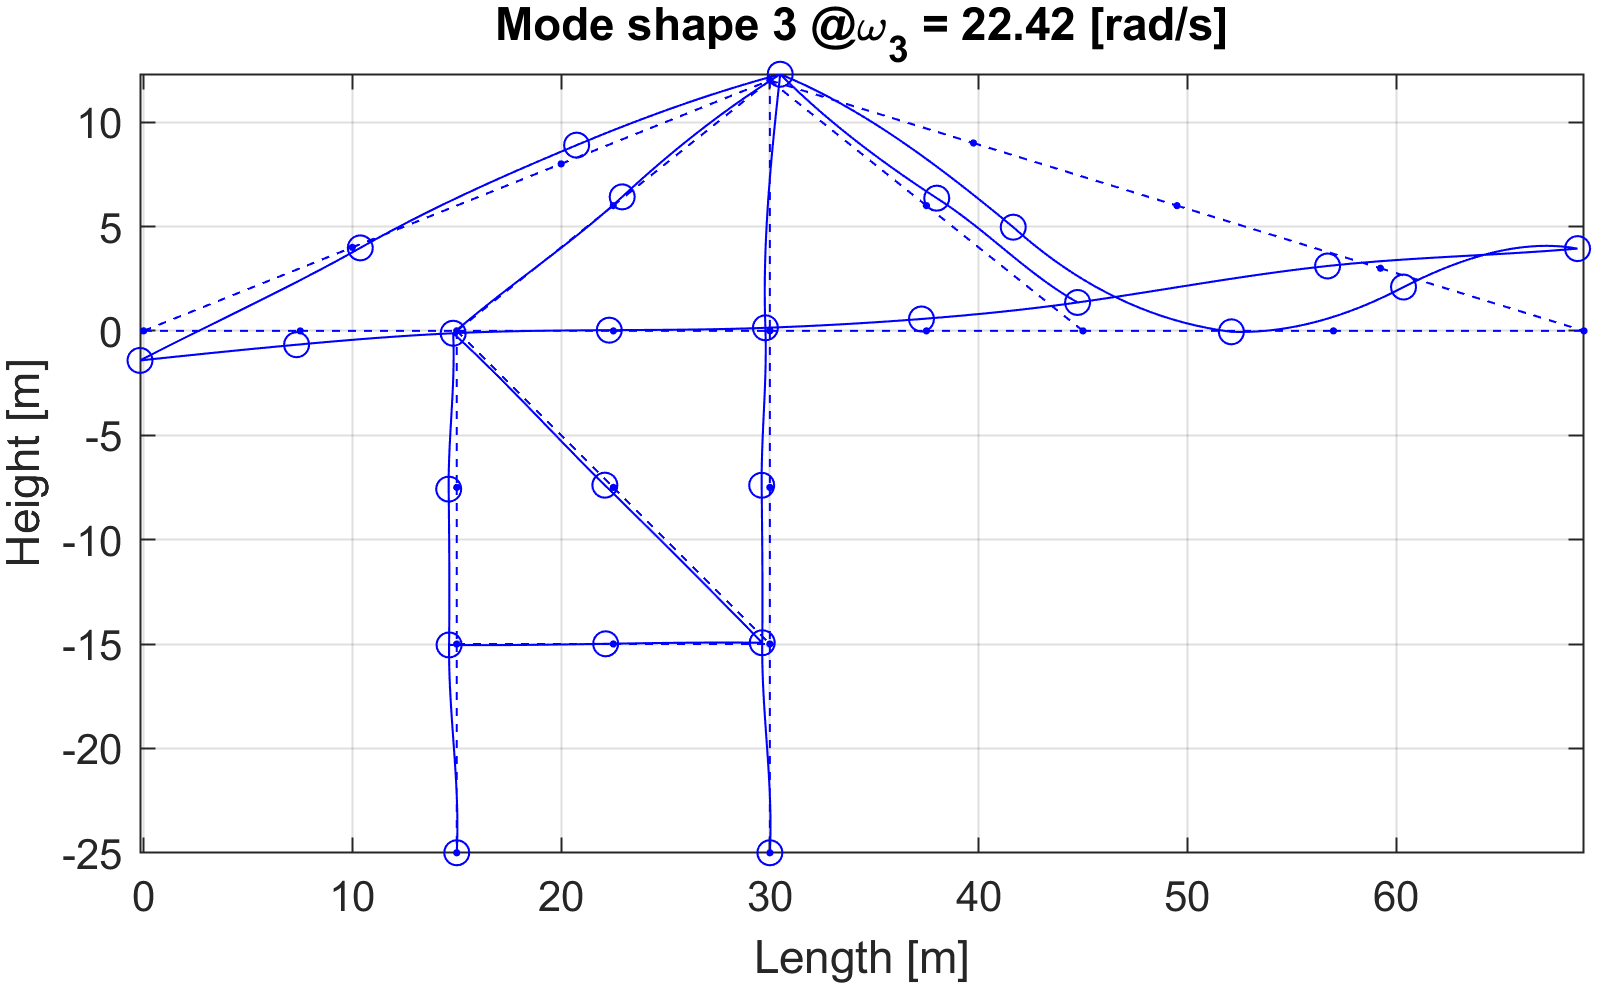
\includegraphics[width=\textwidth]{img/MATLAB/ModeShapes/Mode_03.png}
    \end{minipage}
    \hfill
    \begin{minipage}[b]{0.45\textwidth}
        \centering
        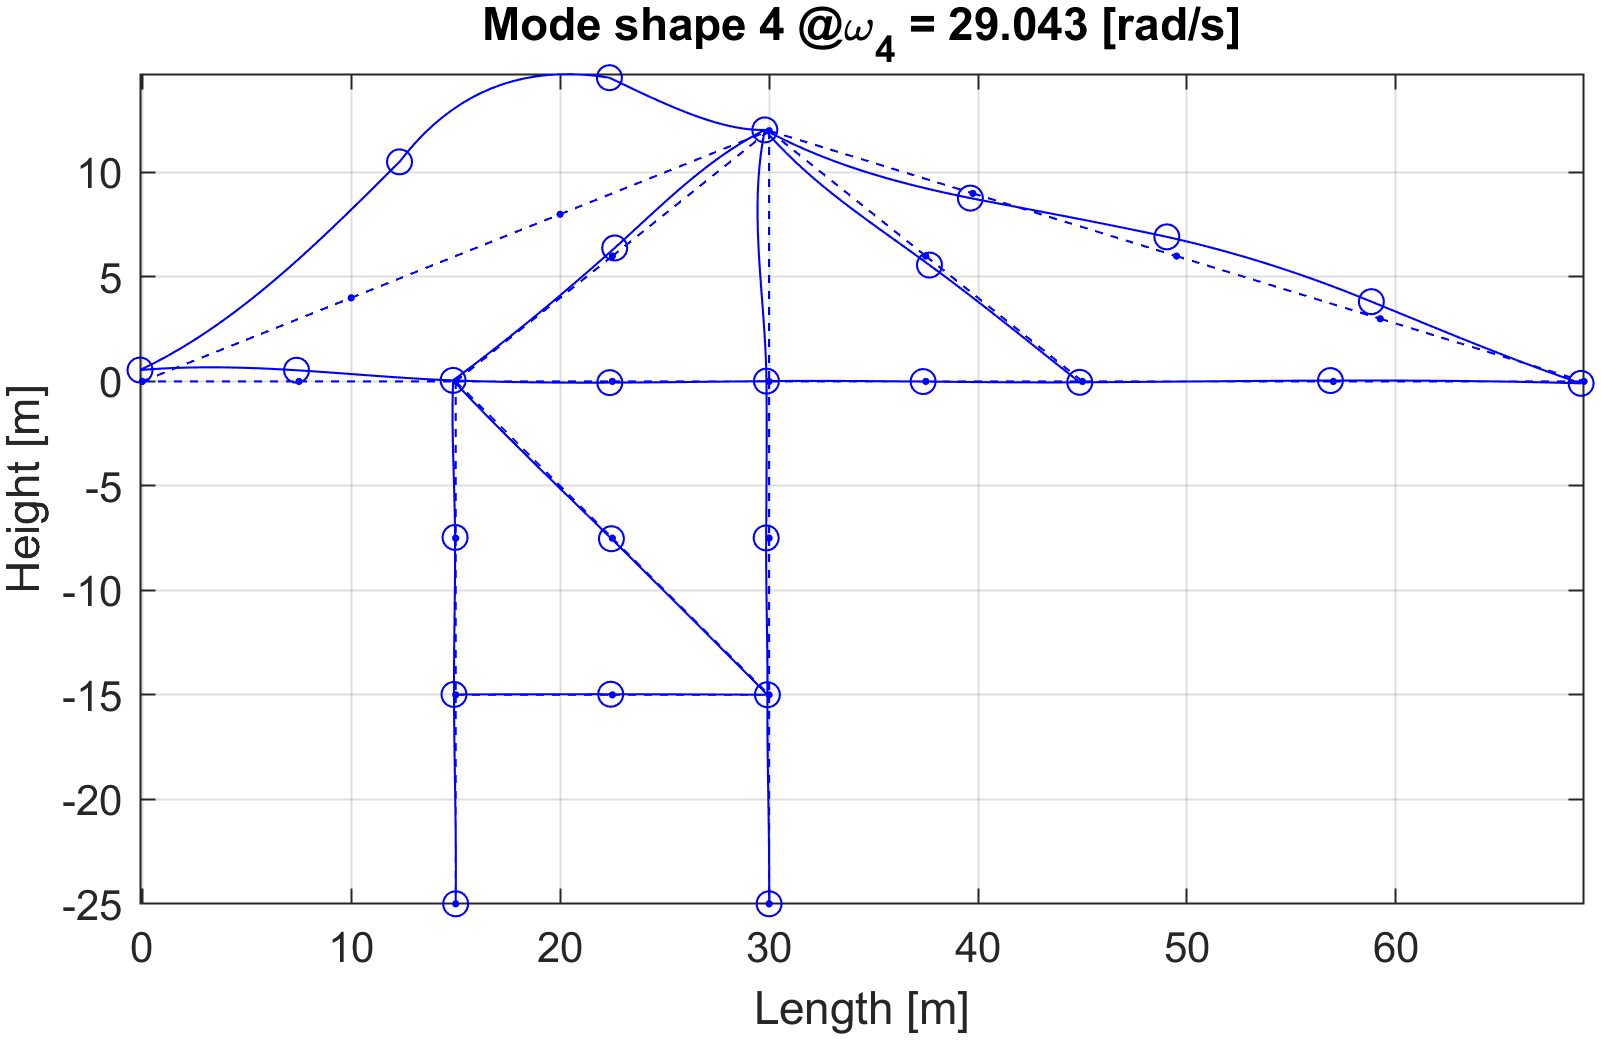
\includegraphics[width=\textwidth]{img/MATLAB/ModeShapes/Mode_04.png}
    \end{minipage}
    \caption{Firsts mode shapes of the FE model}
    \label{fig:mode_shapes}
\end{figure}

\begin{center}
    \huge{The following reasoning is the most interesting of the whole report but must be revised and rewritten in a more straightforward way.}
\end{center}

Notice how the first mode shape is almost a rigid body motion, while the others are more complex and involve bending of the beams.
This can be easily explained by the fact that the equivalent stiffness of the first mode shape is due to only the lateral displacement of the two supporting beam elements that connect the structure to the ground.
This, however, won't be a real problem given that this mode shape is generally not excited by the forces acting on the crane that are usually in the vertical direction.

When we will perform the dynamic analysis of the system, we will see that the mode shapes involved in the response of the system are from the second one on, since they involve the bending of the beams, which is the main source of flexibility of the structure and the one that is directly excited by the vertical forces along the arm of the crane.